\documentclass[a4paper]{article}
\usepackage[utf8]{inputenc}
\usepackage[T1]{fontenc}
\usepackage[english,french]{babel}
\usepackage{amsmath}
\usepackage{amssymb,amsfonts,textcomp}
\usepackage{color}
\usepackage{array}
\usepackage{supertabular}
\usepackage{hhline}
\usepackage{hyperref}
\usepackage{capt-of}
\usepackage[pdftex]{graphicx}
\usepackage{sectsty}
\usepackage{tcolorbox}
\usepackage{textcomp}
\usepackage{courier}
\usepackage[font={small,it}]{caption}
\usepackage{float}
\usepackage{graphicx}
\usepackage{subcaption}
\usepackage{tabularx}



\definecolor{havelockBlue}{rgb}{0.004, 0.42, 0.73}
\definecolor{Monokaimagenta}{rgb}{0.86,0.08,0.24}
\sectionfont{\color{havelockBlue}}

\begin{document}


\begin{titlepage}
	\centering
	
	{\scshape\LARGE \color{Monokaimagenta} Laboratoire \\ L'Unité Arithmétique et Logique (ALU) \par}
	\vspace{1cm}
	
	{\Large\itshape Yohann Meyer \& Sven Rouvinez\par}
	\vfill
	Professeur\par
	\textbf{Carlos Andrés Pena}\par
	\vspace{1cm}
	Assistant\par
	\textbf{Gaëtan Matthey}
	
	\vfill

% Bottom of the page
	{\large \today\par}
\end{titlepage}



\section{Description générale}
\paragraph{}
Il s’agit dans ce laboratoire d’implémenter une ALU à 4 bits. L’ALU effectue 15 opérations arithmétiques et logiques, classés en quatre fonctionnalités. La table détaille ces opérations ainsi que leurs codes (Opcode).

	
\begin{tcolorbox}[colframe=Monokaimagenta,colback=white]
Réponses à diverses questions - Max 1/4 page 
Il est demandé de: 
a. Identifiez les bits de “l’opcode” (op) déterminant la fonctionnalité à exécuter
b. Identifiez pour chaque fonctionnalité les bits de “l’opcode” (op) qui sélectionnent l’opération à exécuter
Remplacez le texte ci-dessus par vos réponses (à l’intérieur du cadre rouge)\\
\begin{center}
    
\begin{tabular}{ l | c |r }
    \hline
    Opcode           &  Fonctionnalité & Opération\\
    \hline
    0000$\phi\phi$   &     \nameref{add_Sub}    & $A+B$ (signé) \\
    0010$\phi\phi$   &                 & $A-B$ (signé) \\
    0001$\phi\phi$   &                 & $A+B$ (non signé) \\
    0011$\phi\phi$   &                 & $A-B$ (non signé) \\
    \hline
    011001           &  \nameref{comp} & $A \ge B$ (signé) \\
    011010           &                 & $A < B$ (signé) \\
    011011           &                 & $A \ne B$\\
    011100           &                 & $A = B$ \\
    011101           &                 & $A \ge B$ (non signé) \\
    011110           &                 & $A < B$ (non signé) \\
    \hline
    10$\phi\phi$00   &\nameref{logique}& $A$ and $B$\\
    10$\phi\phi$01   &                 & $A$ or $B$\\
    10$\phi\phi$10   &                 & $A$ nand $B$\\
    10$\phi\phi$11   &                 & $A$ xor $B$\\
    \hline
    11$\phi\phi\phi$ & \nameref{custom}& Somme des \textbf{1} dans \textbf{B} et \textbf{A}
     
\end{tabular}

\end{center}

\end{tcolorbox}

\section{Architecture}
L’architecture générale de l’ALU est composée de 4 blocs fonctionnels comme illustré dans la figure ci-dessous. Ces blocs, réalisant chacun une fonctionnalité différente, sont conçus, réalisés et testés en simulation sur Logisim. Ensuite, les quatre blocs sont intégrés selon le schéma bloc de la figure et, finalement, ils sont synthétisés et programmés et leur fonctionnement est validé sur la carte Max V. 

\section{Réalisation}
\subsection{Le bloc Add/Sub} \label{add_Sub}

\paragraph{Conception}
Selon le cahier de charges: “Le bloc Add/Sub génère une sortie R[3:0] à 4 bits avec la somme ou la différence entre A et B, ainsi que quatre sorties à 1 bit indiquant, respectivement, en cas de dépassement de capacité (overflow), s’il y a une retenue (carry), si le résultat de l’opération Add/Sub est zéro (zero), et le bit de poids fort du résultat de l’additionneur/soustracteur (R[3])”. Comme entrées au bloc, en plus des opérandes A et B, deux signaux à 1 bit indiquent, respectivement, le type d’opération (Add ou Sub) et le type d’arithmétique (Signée ou Non-signée). Le circuit qui réalise le bloc Add/Sub en respectant les consignes est présenté ci-dessous.\\


\begin{tcolorbox}[colframe=Monokaimagenta,colback=white]
Conception - Max 1 page 
Insérez une capture d’écran pour présenter votre bloc Add/Sub.
Accompagnez-le de commentaires et/ou d’explications nécessaires à sa compréhension.
Remplacez le texte ci-dessus par vos réponses (à l’intérieur du cadre rouge)
\end{tcolorbox}

\begin{tcolorbox}[colframe=Monokaimagenta,colback=white]

\begin{figure}[H]
    \centering
    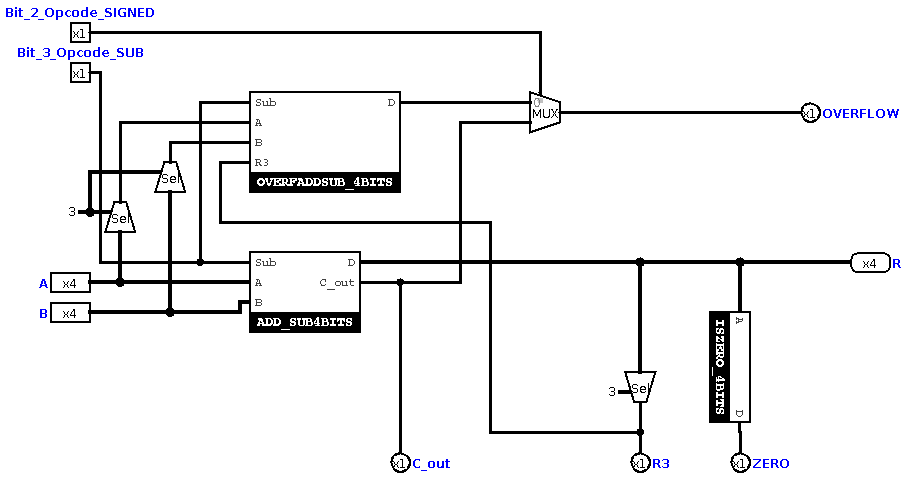
\includegraphics[width=\textwidth]{src/ADDSUB_ALU.png}
    \captionof{figure}{Bloc Add/Sub}
\end{figure}

\paragraph{Définition des entrées}
\begin{itemize}
\item \textbf{Bit\_2\_Opcode\_SIGNED} (1 bit)
     \begin{itemize}
            \item 0 le bloc utilisera des nombres non-signés
            \item 1 le bloc utilisera des nombres signés
        \end{itemize}
\item \textbf{Bit\_3\_Opcode\_SUB} (1 bit) 
    \begin{itemize}
            \item 0: la réponse résultera d'une addition
            \item 1: la réponse résultera d'une soustraction
        \end{itemize}
\item \textbf{A} (4 bits) nombre utilisé pour le calcul 
\item \textbf{B} (4 bits) nombre utilisé pour le calcul 
\end{itemize}

\paragraph{Définition des sorties}
\begin{itemize}
    \item \textbf{OVERFLOW} (1 bit): retourne 1 si le résultat \textbf{A} et \textbf{B} est un dépassement de mémoire. Voir \ref{fig:OVERFADDSUB_4BITS}
    \item \textbf{C\_out} (1 bit): correspond au carry (retenue) du résultat \textbf{A} et \textbf{B}
    
    \item $R_3$ (1 bit): permet de savoir si le bit de poids fort ($R_3$) est actif 
    \item \textbf{ZERO}  (1 bit): permet de savoir si \textbf{A} et \textbf{B} sont les 2 égal à 0. Voir \ref{fig:ISZERO}
\end{itemize}
    
\end{tcolorbox}
\paragraph{Tests} 
Le fonctionnement du circuit Add/Sub est validé au moyen de plusieurs tests effectués en  simulation sur Logisim. Les cas de test sont choisis de façon à illustrer le comportement du circuit dans le plus grand nombre possible de conditions de fonctionnement permettant de vérifier la justesse du résultat et la validité des signaux de sortie: carry, overflow et zero. Ces tests sont présentés à continuation.\\

\begin{tcolorbox}[colframe=Monokaimagenta,colback=white]
Tests - Max 2 pages 
Insérez  un tableau montrant les résultats des tests, illustré avec une ou deux captures d’écran. Privilégiez l’illustration de plusieurs tests sur une même image (vous pouvez aussi utiliser un chronogramme)
Expliquez/justifiez le choix des tests effectués et les résultats obtenus.
Au besoin, ajoutez des annotations textuelles ou graphiques directement sur les images.
Remplacez le texte ci-dessus par vos réponses (à l’intérieur du cadre rouge)
\end{tcolorbox}

\begin{tcolorbox}[colframe=Monokaimagenta,colback=white]
Les tests ci-dessous traite des cas d'additions et soustractions entre nombres signés.\\
\begin{center}


\begin{tabular}{|c|c|c|c||c|c|c|c|c|}
    \hline
     ° & $Op_1$ & A[3:0] & B[3:0] & OVER & $C_{out}$ & $R_3$ & ZERO & Rés. \\
    \hline
    1  & 00     & 0101   & 1010   & 0    &  0        &   1   &  0   & 1010\\
    2  &        & 1101   & 1010   & 1    &  1        &   0   &  0   & 0111 \\
    \hline
    3  & 10     & 1001   & 1001   & 0    &  1        &   0   &  1   & 0000\\
    4  &        & 0111   & 1111   & 1    &  0        &   1   &  0   & 0110\\
    \hline
    
\end{tabular}



\end{center}
\paragraph{$A+B$ (signés)}
Les tests 1 et 2 démontre que le bloc fonctionne correctement lors d'une addition de 2 nombres signés.\\
Le premier montre comment fonctionne $R_3$, en effet la sortie est active et le bit de poids fort de l'entrée \textbf{B} l'est aussi.\\
Le deuxième illustre comment le système se comporte lorsque sa limite est atteinte. Les sorties \textbf{OVERFLOW} et $C_{out}$ sont bel et bien actives.
\begin{figure}[H]
    \centering
    
    \begin{subfigure}{.7\textwidth}
        \centering
        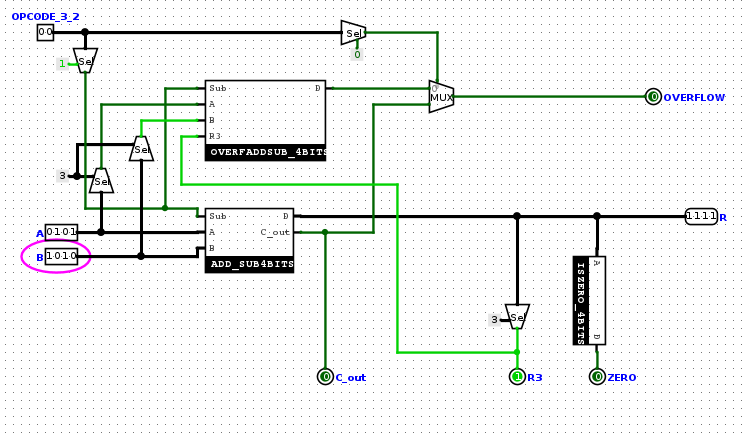
\includegraphics[width=.8\linewidth]{src/ADDSUB_TEST_AplB.png}
        \label{fig:COMPARATEUR_EXEMPLE}
   \end{subfigure}
   
   \begin{subfigure}{.7\textwidth}
        \centering
        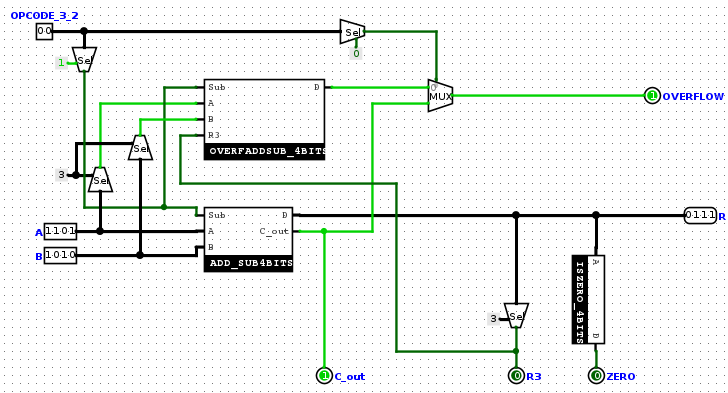
\includegraphics[width=.8\linewidth]{src/ADDSUB_TEST_AplB1.png}
        \label{fig:COMPARATEUR_EXEMPLE_1}
   \end{subfigure}

\captionof{figure}{Exemple $A + B$ (signés)}

\end{figure}

\paragraph{$A-B$ (signés)}
Les tests 3 et 4 Les tests 1 et 2 démontre que le bloc fonctionne correctement lors d'une soustraction de 2 nombres signés.\\
Le troisième permet de comprendre le fonctionnement de la sortie ZERO, en effet lorsque 2 nombres négatifs égaux sont soustrait, le résultat sera 0000.\\
Le test suivant gère un overflow avec la sortie $R_3$ aussi active car le résultat est faussé par le dépassement, d'où l'importance du 1 dans la sortie OVEFLOW.


\end{tcolorbox}

\begin{tcolorbox}[colframe=Monokaimagenta,colback=white]

\begin{figure}[H]
    \centering
    
    \begin{subfigure}{.7\textwidth}
        \centering
        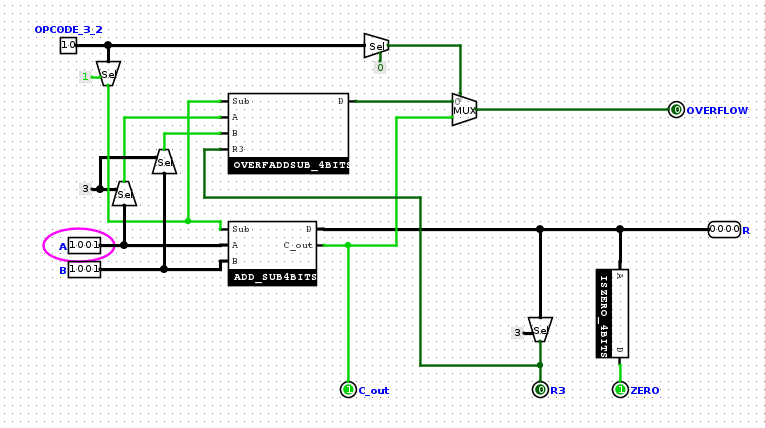
\includegraphics[width=.8\linewidth]{src/ADDSUB_TEST_AmoB.png}
        \label{fig:COMPARATEUR_EXEMPLE}
   \end{subfigure}
   
   \begin{subfigure}{.7\textwidth}
        \centering
        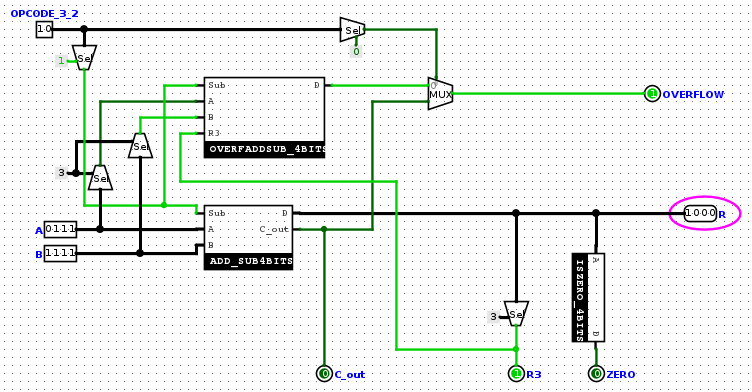
\includegraphics[width=.8\linewidth]{src/ADDSUB_TEST_AmoB1.png}
        \label{fig:COMPARATEUR_EXEMPLE_1}
   \end{subfigure}

\captionof{figure}{Exemple $A - B$ (signés)}


\begin{tabular}{|c|c|c|c||c|c|c|c|c|}
    \hline
     ° & $Op_1$ & A[3:0] & B[3:0] & OVER & $C_{out}$ & $R_3$ & ZERO & Rés. \\
    \hline
    5  & 01     & 0100   & 1101   & 1    &  1        &   0   &  0   & 0001\\
    \hline
    
\end{tabular}

\paragraph{$A+B$ (non signés)}
Le 5ème cas se différence du premier car l'utilisation de non-signés permet d'élargir l'intervalle de valeurs représentable. Avant il y avait $2^3$ possibilités et maintenant il y a $2^4$ donc un overflow va sur survenir mais cette fois à partir de 16.\\


\paragraph{$A-B$ (non signés)}
Les tests intéressants ont été couverts par ceux d'avant. \\

\begin{figure}[H]
    \centering
    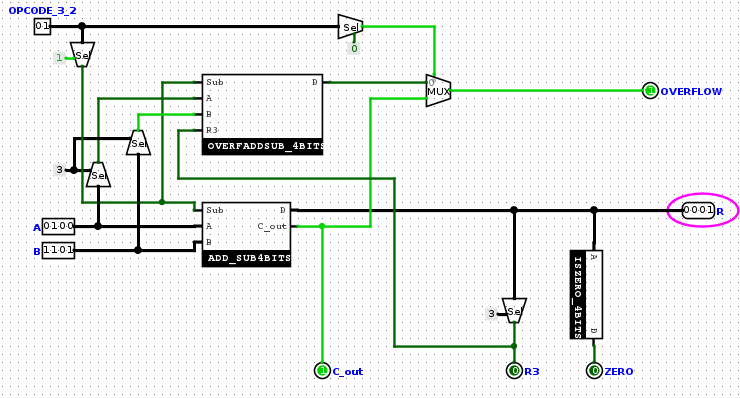
\includegraphics[width=\textwidth]{src/ADDSUB_TEST_AmoNsB.png}
    \captionof{figure}{Bloc OVERFLOW}
    \label{fig:OVERFADDSUB_4BITS}
\end{figure}

\end{figure}


\end{tcolorbox}

\begin{tcolorbox}[colframe=Monokaimagenta,colback=white]
Réponses à diverses questions - Max 1 page
Expliquez brièvement la logique derrière le calcul d’overflow (dépassement) dans les différents cas (signé ou non-signé, addition ou soustraction.
Quelles sont les valeurs maximum et minimum des opérandes ou du résultat que l’on peut obtenir sans qu’il y ait une erreur d’opération?
Remplacez le texte ci-dessus par vos réponses (à l’intérieur du cadre rouge)
\end{tcolorbox}

\begin{tcolorbox}[colframe=Monokaimagenta,colback=white]

\begin{figure}[H]
    \centering
    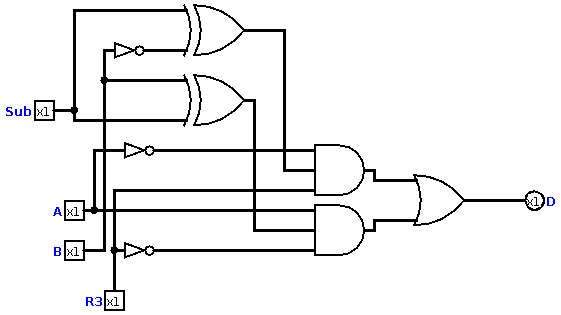
\includegraphics[width=\textwidth]{src/OVERFADDSUB_4BITS}
    \captionof{figure}{Bloc OVERFLOW}
    \label{fig:OVERFADDSUB_4BITS}
\end{figure}

\paragraph{Calcul de l'overflow}
    L'addition et la soustraction de nombres signés se comporte différement car sur 4 bits, 1 bit est utilisé pour le signe du nombre et donc les 3 restant seront utilisé pour la représentation du chiffre voulu. C'est pour cela que lors d'une addition de 2 nombres signés dont le resultat dépasse, nous nous retrouvons avec un nombre négatif.\\
    Intervalle de valeurs représentable: $-7$ à $7$
    \subparagraph{Exemples:} $0110 + 0011 = 1001$ il y a donc 3 bits, de 0 à 7  disponible pour représenter les nombres, ici $0110 = 6$ et $0011 = 3$ mais le résultat étant $9$, l'invervalle des valeurs représentable ne comprend la réponse.\\
    Avec une soustraction: $1011 - 0101  = 0000$ car $-3 - 5 = -8$\\
    
    
\paragraph{Opérandes MAX signées} TODO

Les valeurs maximum pouvant être représentées sont -7 et 7
    \begin{tabular}{|c|c|c|}
   
    
\end{tabular}        
        
\end{tcolorbox}

\subsection{Le bloc Comparateur}
\label{comp}
\paragraph{Conception} Selon le cahier de charges, le comparateur utilise trois signaux en provenance du bloc Add/Sub: la retenue (carry), la détection de zéro (zero), et le bit de poids fort du résultat (R[3]) en plus de quelques bits sélectionnées des entrées A, B, et op. La sortie cmp est active (c’est à dire d’une valeur égale à 0001) selon la logique ci-dessous.

\begin{tcolorbox}[colframe=Monokaimagenta,colback=white]
Conception - Max 1 page 
Insérez une capture d’écran pour présenter votre bloc Comparateur. 
Annotez votre capture et accompagnez-la de commentaires et/ou d’explications nécessaires à sa compréhension.
Remplacez le texte ci-dessus par vos réponses (à l’intérieur du cadre rouge)
\end{tcolorbox}

\begin{tcolorbox}[colframe=Monokaimagenta,colback=white]

\begin{figure}[H]
    \centering
    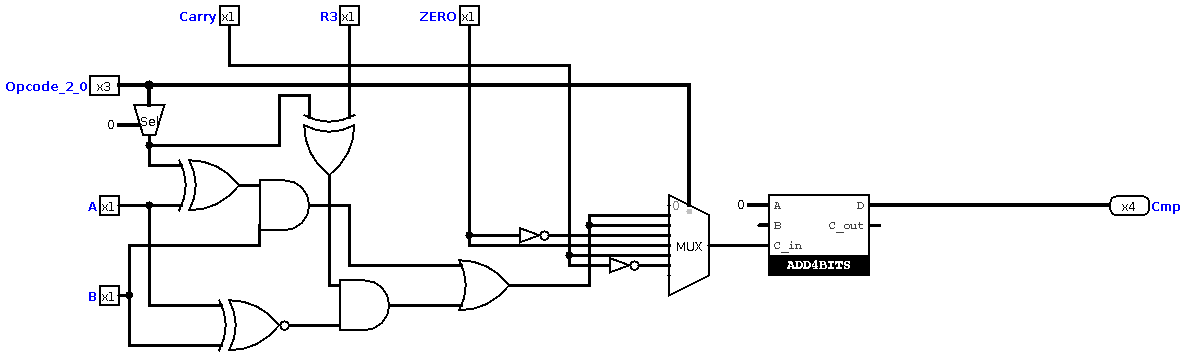
\includegraphics[width=\textwidth]{src/COMPATEUR.png}
    \captionof{figure}{Bloc COMPARATEUR}
    \label{fig:OVERFADDSUB_4BITS}
\end{figure}

\paragraph{Définition des entrées}
Elles sont obtenues selon le résultats du bloc Add/Sub
\begin{itemize}
\item \textbf{Carry} (1 bit)
     \begin{itemize}
            \item 0: s'il n'y a pas de retenue
            \item 1: s'il y a une retenue
        \end{itemize}
\item \textbf{Opcode\_2\_0} (3 bits) définit l'opération choisie
     \begin{itemize}
            \item \begin{tabular}{ |l | l| }
                    001   & $A \ge B$ (signé) \\
                    010   & $A < B$ (signé) \\
                    011   & $A \ne B$\\
                    100   & $A = B$ \\
                    101   & $A \ge B$ (non signé) \\
                    110   & $A < B$ (non signé) \\
    \end{tabular}
        \end{itemize}
\item $R_3$ (1 bit) 
\begin{itemize}
            \item 0: aucun bit de poids fort actif
            \item 1: un bit de poids fort actif
        \end{itemize}
\item \textbf{ZERO} (1 bit) 
    \begin{itemize}
            \item 0: le résultat n'est pas égal à \textbf{0}
            \item 1: le résultat est égal à \textbf{0}
        \end{itemize}
\item \textbf{A} (1 bit) nombre utilisé pour le calcul, utilisation du bit de poids fort
\item \textbf{B} (1 bit) nombre utilisé pour le calcul, utilisation du bit de poids fort
\end{itemize}

\paragraph{Définition de la sortie}
La sortie du bloc est ensuite transmise à un circuit qui nous permet d'additionner afin d'obtenir une sortie sur 4 bits comme voulue.\\
Les résultats attendus sont: 
\begin{itemize}
 \item    0000 si la comparaison est fausse, par exemple $A \ngeq B$
 \item    0001 si la comparaison est correcte, par exemple $A = B$
\end{itemize}
L'utilisation d'un "Bit selector" permet de sélectionner le type de comparaison voulue, ce plexer va "couper" notre opcode qui sera équivalent à \textbf{011XXX} et de choisir uniquement les 3 bits qui nous intéressent. Par exemple si l'opération voulue est $A=B$(100), nous allons donc prendre le groupe 4, le groupe 0 serait égal à \textbf{000} et le groupe 1 à \textbf{001}.\\
L'utilisation de MUX permet d'aiguiller le résultat selon les tests effectués et de retourner \textbf{1} si la comparaison est correcte ou \textbf{0} si elle est fausse.

\end{tcolorbox}

\begin{tcolorbox}[colframe=Monokaimagenta,colback=white]
Réponses à diverses questions (max 1/2 page)
Expliquez clairement les fonctions logiques de comparaison qui vous ont été fournies dans le tableau ci-dessus derrière le bloc comparateur 
Dans quels cas le résultat de la comparaison ne peut, ou ne doit, pas être utilisé à cause d’une erreur d’opération? Justifiez votre réponse.
Remplacez le texte ci-dessus par vos réponses (à l’intérieur du cadre rouge)

TODO: Dans quels cas le résultat de la comparaison ne peut, ou ne doit, pas être utilisé à cause d’une erreur d’opération? 

\paragraph{$A \ge B$ (signé)} (not(A[3]) and B[3]) or (not(R[3]) and (A[3] xnor B[3]))\\
Cette opération utilise uniquement les bits de poids de fort des entrées selon la consigne.
Si \textbf{A} ou \textbf{B} sont actifs, ils seront négatif.\\
Une porte AND sera toujours fausse si une entrée est différente à 1 donc dans le cas oû les 2 entrées sont à 0 ou l'une différente de l'autre le résultat de comparaison sera faux quelque soit le reste de l'opération. Une porte XNOR est vrai lorsque les 2 valeurs sont vraies ou fausses et ensuite la porte AND va nous permettre de retourner vrai uniquement si R est faux et la sortie du XNOR est vrai.

\paragraph{$A < B$ (signé)} (A[3] and not(B[3])) or (R[3] and (A[3] xnor B[3]))\\
Si \textbf{A} ou \textbf{B} sont actifs, ils seront négatif.\\
Le bit de poids fort va nous permettre de savoir quand $A<B$ lorsque les 2 sont négatifs donc si $R_3=1$ cela va nous avertir que  $A<B$ et dans le cas contraire le résultat de l'opération (R[3] and (A[3] xnor B[3]) sera égale à 0 et donc la comparaison sera fausse.

\paragraph{$A=B$} not(zero)\\
Grâce au bloc Add/Sub, si le résultat vaut 0 nous sommes directement en mesure de traiter le signal pour savoir s'il est actif ou pas.

\paragraph{$A=B$} zero\\
Même fonctionnement que le paragraphe ci-dessus mais avec la différence que la porte NOT n'est pas utilisée car cette fois le système doit afficher si c'est égale à 0.

\paragraph{$A \ge B$ (non signés)} carry\\
La retenue nous permet définir s'il y a un dépassement de mémoire

\paragraph{$A < B$ (non signés)} not(carry)\\
Si l'entrée carry n'est pas activée cela revient à dire que l'opération s'est déroulée correctement


\end{tcolorbox}

\paragraph{Tests}
Le correct fonctionnement du comparateur est vérifié par quelques tests, sélectionnés de façon à illustrer clairement le résultat des opérations de comparaison avec différentes valeurs d’opérandes. Les figures suivantes montrent les tests qui ont été réalisés.

\begin{tcolorbox}[colframe=Monokaimagenta,colback=white]
Tests - Max 1 page 
Insérez  un tableau montrant les résultats des tests, illustré avec une ou deux captures d’écran. Privilégiez l’illustration de plusieurs tests sur une même image (vous pouvez aussi utiliser un chronogramme)
Expliquez/justifiez le choix des tests effectués et les résultats obtenus.
Au besoin, ajoutez des annotations textuelles ou graphiques directement sur les images.
Remplacez le texte ci-dessus par vos réponses (à l’intérieur du cadre rouge)\\
TODO REPLACEZ IMAGES
\begin{center}
    
    \begin{figure}[H]
    \centering
    
    \begin{subfigure}{.7\textwidth}
        \centering
        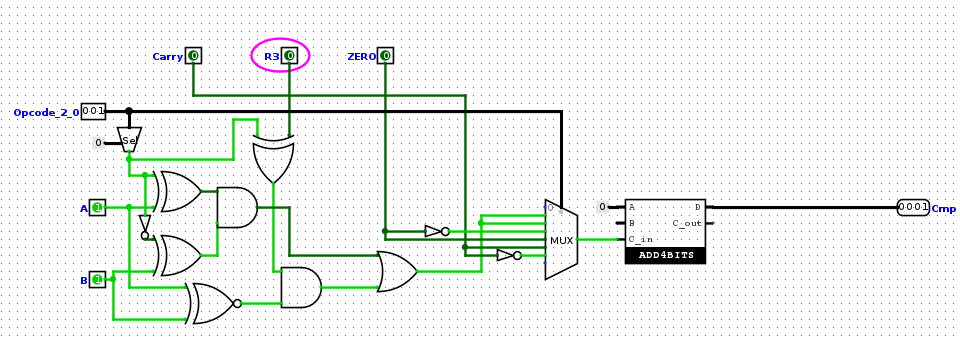
\includegraphics[width=.8\linewidth]{src/COMP_TEST_AgeB.png}
        \label{fig:COMPARATEUR_EXEMPLE}
   \end{subfigure}
   
   \begin{subfigure}{.7\textwidth}
        \centering
        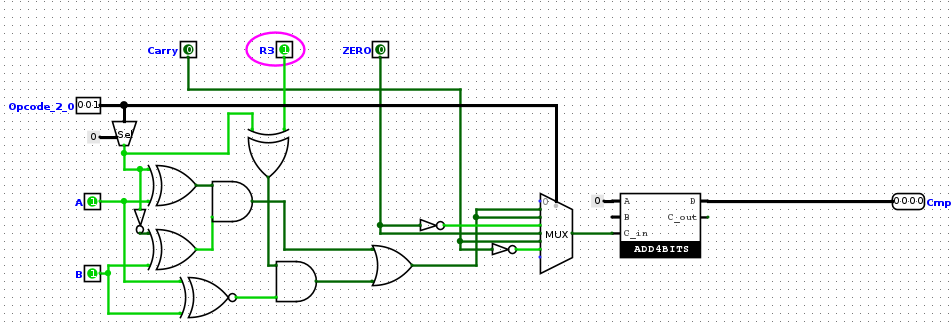
\includegraphics[width=.8\linewidth]{src/COMP_TEST_AgeB1.png}
        \label{fig:COMPARATEUR_EXEMPLE_1}
   \end{subfigure}

\captionof{figure}{Exemple COMPARATEUR $A\ge B$}

\end{figure}
    
    Un résultat interéssant est quand \textbf{A} (1) est négatif et \textbf{B} (1) avec $R_3$ qui n'est pas activé afin de montrer son importance. Voir images ci-dessus
\begin{tabular}{|c|c|c|c|cc|}
\hline
    Opcode & A & B & $R_3$ & $\overline{A} B + \overline{R_3}(\overline{A \oplus B})$ & Circuit\\
   \hline
    001    & 1 & 1 & 0     & 1             & 1 \\           
           & 1 & 1 & 1     & 0             & 0 \\
    \hline
\end{tabular}

\smallskip
    
    \begin{figure}[H]
    \centering
    
    \begin{subfigure}{.7\textwidth}
        \centering
        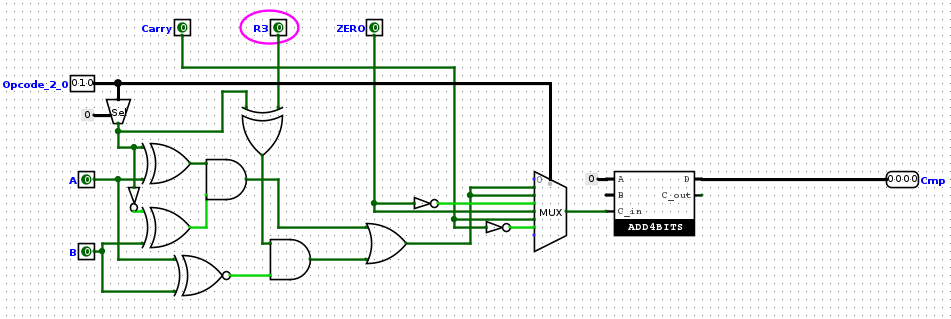
\includegraphics[width=.8\linewidth]{src/COMP_TEST_AlB.png}
        \label{fig:COMPARATEUR_l_EXEMPLE}
   \end{subfigure}
   
   \begin{subfigure}{.7\textwidth}
        \centering
        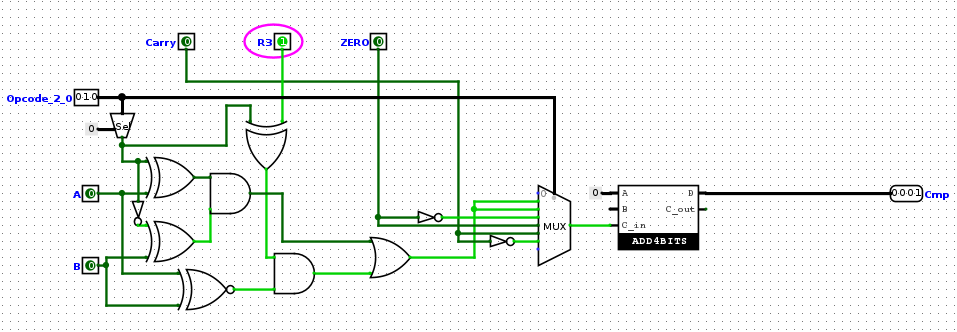
\includegraphics[width=.8\linewidth]{src/COMP_TEST_AlB1.png}
        \label{fig:COMPARATEUR_l_EXEMPLE_1}
   \end{subfigure}

\captionof{figure}{Exemple COMPARATEUR $A < B$}

\end{figure}

         


    Lorsque que A est positif et B aussi le bit de poids fort nous permettra de choisir le chiffre le plus grand. Voir images ci-dessus 
\begin{tabular}{|c|c|c|c|cc|}
\hline    
Opcode & A & B & $R_3$ & $A\overline{B} + {R_3}(\overline{A \oplus B})$ & Circuit\\
\hline
    010    & 0 & 0 & 0     & 1             & 1\\
           & 0 & 0 & 1     & 0             & 0\\
    \hline
         
\end{tabular}

\smallskip
\begin{figure}[H]
    \centering
    
    \begin{subfigure}{.7\textwidth}
        \centering
        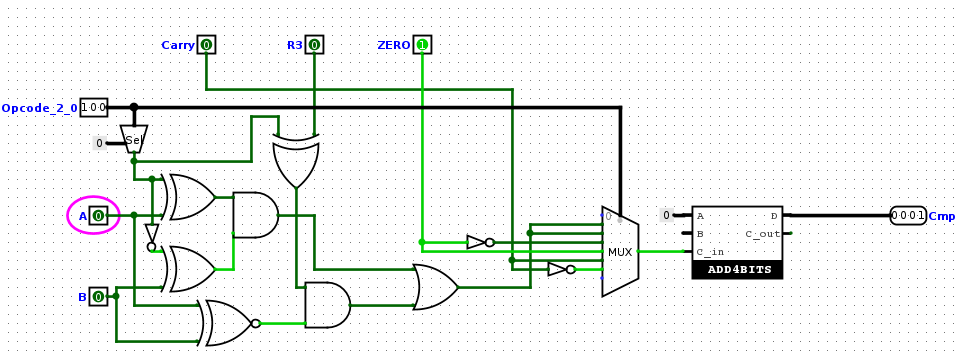
\includegraphics[width=.8\linewidth]{src/COMP_TEST_AegB1.png}
        \label{fig:COMPARATEUR_l_EXEMPLE}
   \end{subfigure}
   
   \begin{subfigure}{.7\textwidth}
        \centering
        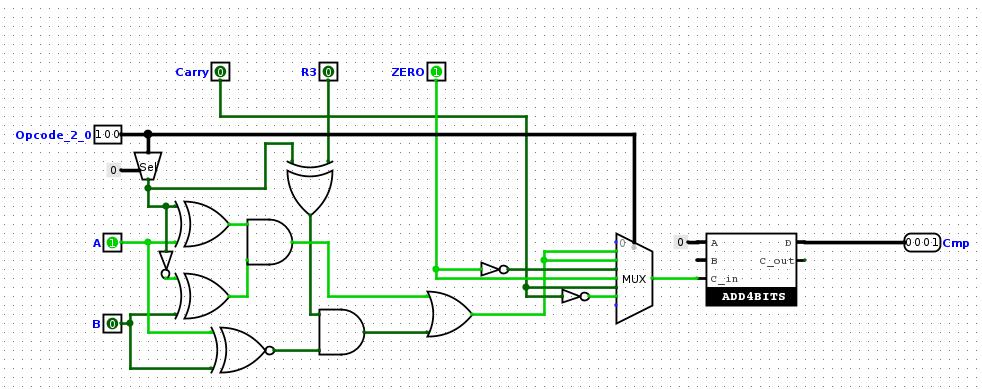
\includegraphics[width=.8\linewidth]{src/COMP_TEST_AegB.png}
        \label{fig:COMPARATEUR_l_EXEMPLE_1}
   \end{subfigure}

\captionof{figure}{Exemple COMPARATEUR $A = B$}

\end{figure}

Si le zero est actif, les entrées \textbf{A} et \textbf{B} sont ignorées car c'est le boc Add/Sub qui donne l'information.\\
Le cas du not(zero) est semblable, il y a juste un inversion logique.

\smallskip

\begin{figure}[H]
    \centering
    
    \begin{subfigure}{.7\textwidth}
        \centering
        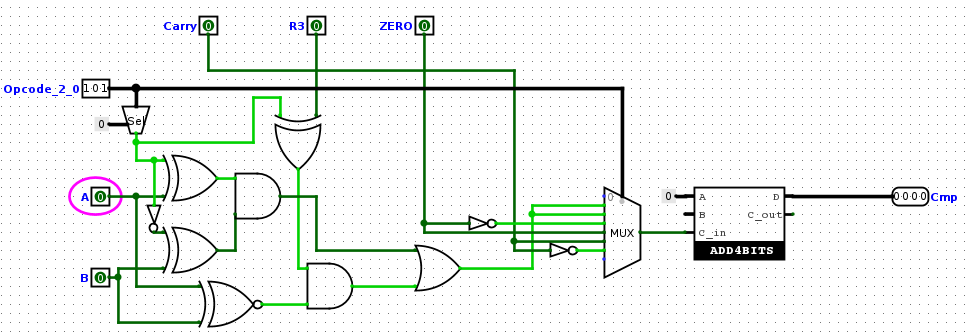
\includegraphics[width=.8\linewidth]{src/COMP_TEST_AcarB.png}
        \label{fig:COMPARATEUR_l_EXEMPLE}
   \end{subfigure}
   
   \begin{subfigure}{.7\textwidth}
        \centering
        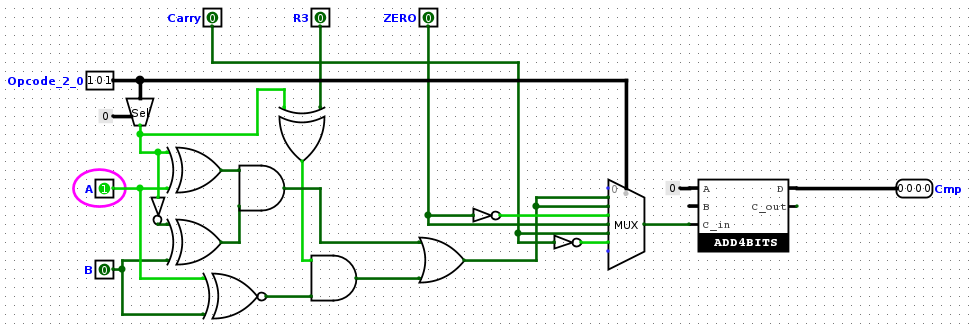
\includegraphics[width=.8\linewidth]{src/COMP_TEST_AcarB1.png}
        \label{fig:COMPARATEUR_l_EXEMPLE_1}
   \end{subfigure}

\captionof{figure}{Exemple COMPARATEUR $A = B$}

\end{figure}

Dans cette comparaison, seule la retenue est  transmise par le bloc Add/Sub l'entrée \textbf{Carry}.\\
Le cas du not(carry) est semblable, il y a juste un inversion logique.



\end{center}

\end{tcolorbox}

\subsection{L'unité logique}
\label{logique}

\paragraph{Conception et tests}
L’unité logique, réalisée en Logisim et montrée dans le schéma ci-dessous, calcule les 4 opérations logiques demandées par le cahier de charges. Les opérations sont effectuées bit à bit entre les deux opérandes.

\begin{tcolorbox}[colframe=Monokaimagenta,colback=white]
Conception et tests - Max 1 page 
Insérez une capture d’écran pour présenter votre unité logique
Accompagnez-les de commentaires et/ou d’explications nécessaires à sa compréhension.
Présentez quelques exemples de tests  afin de pouvoir observer le fonctionnement des opérations logiques.
Remplacez le texte ci-dessus par vos réponses (à l’intérieur du cadre rouge)\\

\end{tcolorbox}

\begin{tcolorbox}[colframe=Monokaimagenta,colback=white]

\begin{figure}[H]
    \centering
    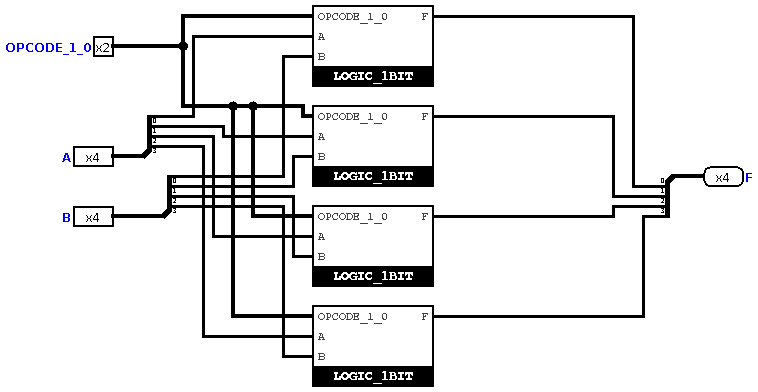
\includegraphics[width=\textwidth]{src/LOGIC_4BITS.png}
    \captionof{figure}{Bloc LOGIQUE}
    \label{fig:LOGIQUE}
\end{figure}


\paragraph{Définition des entrées}
Le calcul se fait bit par bit d'où l'utilisation de splitter pour permettre de transmettre les bits aux circuits responsables.

    \begin{itemize}
    \item     \textbf{OPCODE\_1\_0} (2 bits) sélectionne l'opération logique
    \begin{itemize}
        \item     AND
        \item     OR
        \item     NAND
        \item     XOR
    \end{itemize}
    
    \item \textbf{A} (4 bits) nombre utilisé pour le calcul 
    \item \textbf{B} (4 bits) nombre utilisé pour le calcul 
    \end{itemize}
\paragraph{Définition de la sortie}


    
Les portes NAND sont des portes universelles, c'est-à-dire qu'elles peuvent ensemble, représenter toutes les portes logiques, dans notre cas, elles simulent grâce au circuit LOGIC\_1BIT définit ci-dessous. 
L'utilisation de telles portes se justifie par le coût relativement réduit de ces portes. Une porte NAND coûte ~0.40\$ tandis ce que un porte OR revient à 0.50\$ (http://www.ti.com/)

\begin{figure}[H]
    \centering
    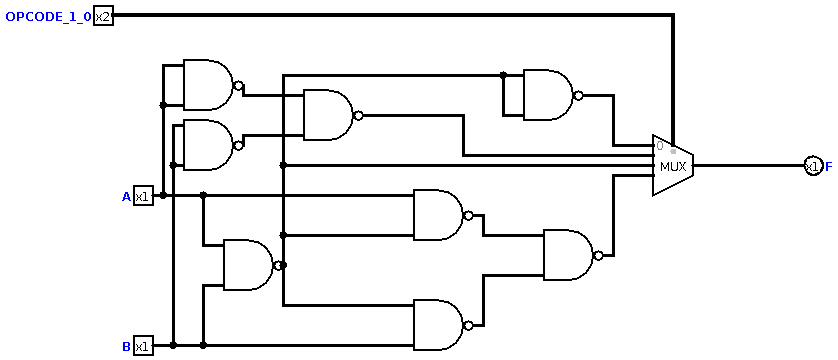
\includegraphics[width=\textwidth]{src/LOGIC_1BIT.png}
    \captionof{figure}{Circuit LOGIQUE 1BIT}
    \label{fig:LOGIQUE_1BIT}
\end{figure}

\end{tcolorbox}



\paragraph{Exemples}


\subsection{Opération custom}
\label{custom}

\paragraph{Conception et tests}
l est demandé de réaliser un circuit qui calcule le nombre total de bits, en A et en B, qui valent 1. Cette opération est effectuée par le système combinatoire de la figure suivante:

\begin{tcolorbox}[colframe=Monokaimagenta,colback=white]
Conception et tests -  Max 1 page 
Insérez une capture d’écran pour présenter votre bloc Custom
Accompagnez-les de commentaires et/ou d’explications nécessaires à sa compréhension.
Expliquez clairement le principe de fonctionnement de votre réalisation de l’opération custom et comment vous avez réussi à réduire le nombre d’additionneurs au minimum.
Présentez quelques exemples de fonctionnement au moyen de simulations sur Logisim
Remplacez le texte ci-dessus par vos réponses (à l’intérieur du cadre rouge)

\begin{figure}[H]
    \centering
    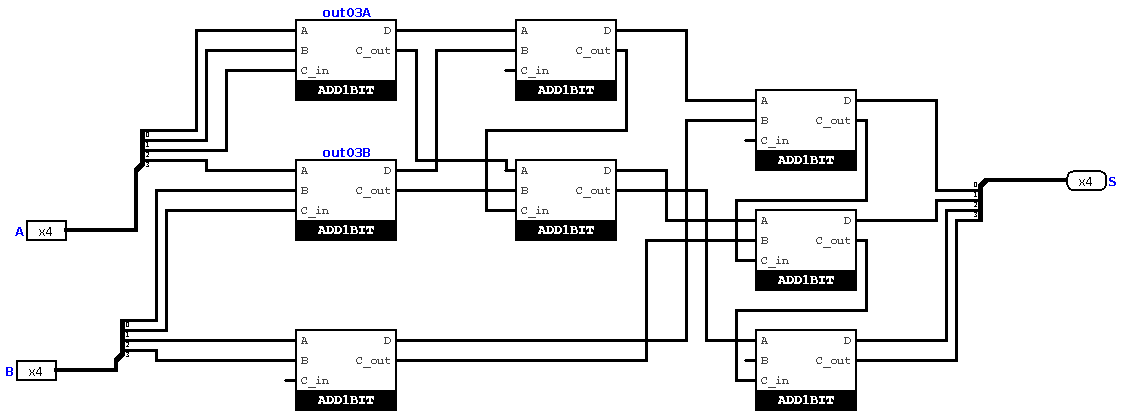
\includegraphics[width=\textwidth]{src/CUSTOM.png}
    \captionof{figure}{Bloc CUSTOM}
    \label{fig:CUSTOM}
\end{figure}

\paragraph{Exemple}
Dans l'image ci-dessous le bloc CUSTOM est activé grâce à l'opcode et l'entrée \textbf{A} vaut 0001 (9) et \textbf{B} vaut 1001 (9) donc notre sortie égale bien 0011 (3)
\begin{figure}[H]
    \centering
    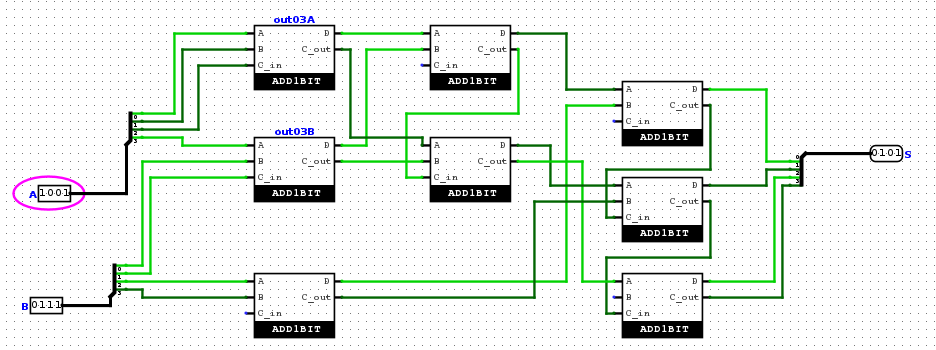
\includegraphics[width=\textwidth]{src/COMP_TEST.png}
    \captionof{figure}{Exemple CUSTOM}
    \label{fig:CUSTOM}
\end{figure}

\begin{figure}[H]
    \centering
    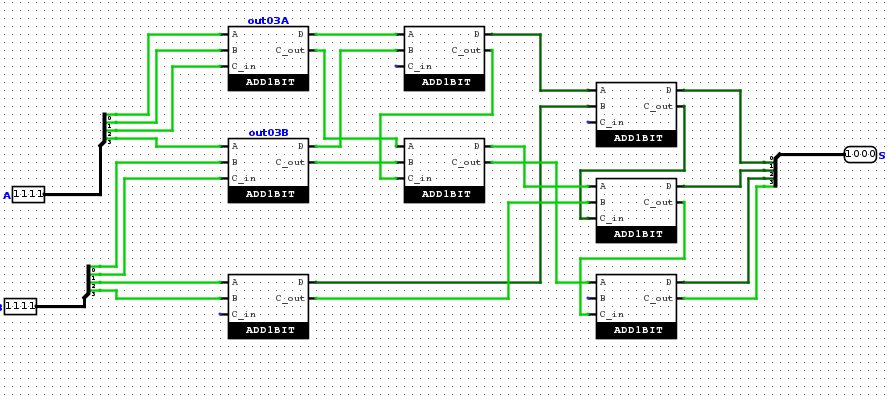
\includegraphics[width=\textwidth]{src/COMP_TEST_1111.png}
    \captionof{figure}{Exemple CUSTOM}
    \label{fig:CUSTOM}
\end{figure}



Le bloc se comporte essentiellement de circuits 1 bit (\ref{fig:ADD_1BIT}) qui vont permettre de contrôler si un bit des entrées est actif ou pas et ensuite d'effectuer une addition.

\end{tcolorbox}

\subsection{Intégration}
\paragraph{Réalisation et tests}
Le schéma ci-dessous montre le circuit Logisim de l’ALU, avec les 4 blocs présentés avant et les circuits permettant (1) de sélectionner le résultat produit par chacun des blocs correspondant à une fonctionnalité et (2) de générer le signal d’erreur selon le cahier de charges. 

\begin{tcolorbox}[colframe=Monokaimagenta,colback=white]
Réalisation et tests - Max 1 page 
Insérez une capture d’écran du schéma-bloc général de votre ALU
A l’aide d’un tableau, donnez un exemple pour chaque bloc correspondant à une fonctionnalité et montrez la pertinence du signal d’erreur par quelques exemples
Remplacez le texte ci-dessus par vos réponses (à l’intérieur du cadre rouge)

\begin{figure}[H]
    \centering
    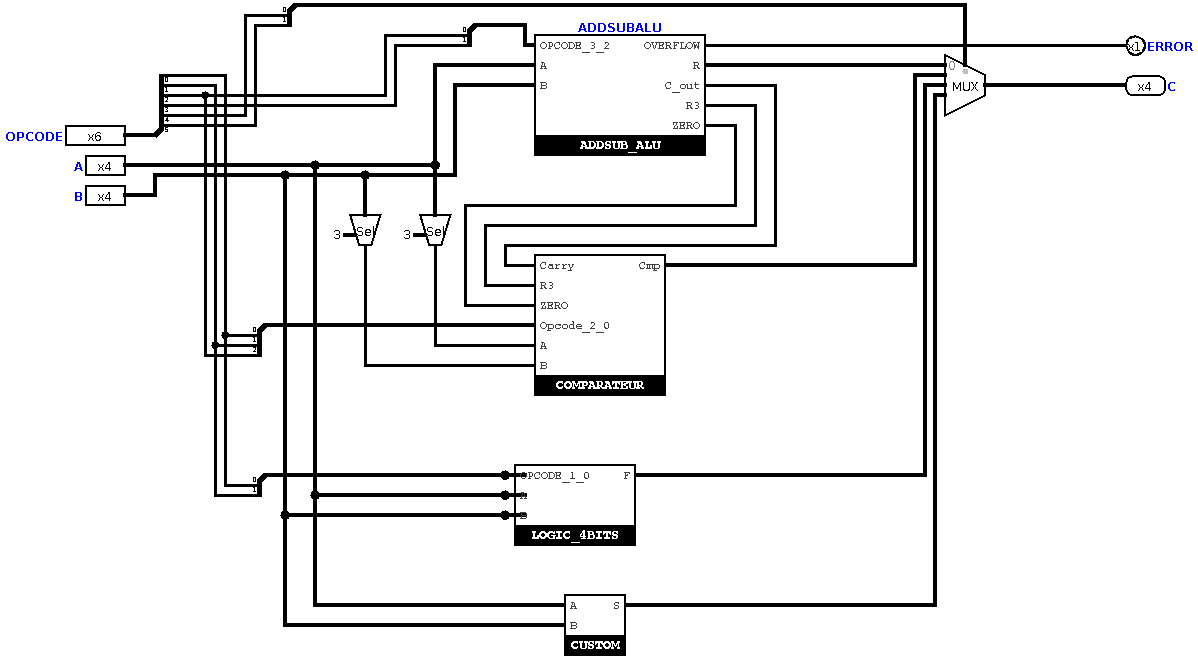
\includegraphics[width=\textwidth]{src/ALU.png}
    \captionof{figure}{ALU}
    \label{fig:ALU}
\end{figure}

L'ALU est composé de 4 quatres blocs:
\begin{itemize}

\item    \nameref{add_Sub} qui permet de faire une addition ou une soustraction
\item    \nameref{comp} qui permet de faire une comparaison entre les bits de poids forts
\item    \nameref{logique} effectue les opérations:
    \begin{itemize}
        \item     AND
        \item     OR
        \item     NAND
        \item     XOR
    \end{itemize}
\item    \nameref{custom} calcul la somme de 1 actif dans \textbf{A} et \textbf{B}

\end{itemize}


\end{tcolorbox}

\subsection{Synthèse et test de fonctionnement réel}
\paragraph{Synthèse et configuration du matériel, test de fonctionnement.}
L’ALU est finalement synthétisée dans le but de configurer (programmer) le circuit programmable présent dans la carte Max V. Les opérandes sont entrés grâce aux interrupteurs de la console. Le code d’opération est sélectionné grâce aux dip-switchs de la carte et le résultat, ainsi que le signal d’erreur, sont affichés au moyen des lampes LED de la console. Cette configuration est testée et quelques exemples sélectionnés sont réalisés pour vérifier la justesse des résultats obtenus et du comportement général du circuit.

\begin{tcolorbox}[colframe=Monokaimagenta,colback=white]
Essais avec une carte - Max 1 page 
Vous devez avoir montré votre circuit en fonctionnement au professeur ou à l’assistant
Illustre cette étape par une photo du circuit en fonctionnement.
Commentez brièvement votre expérience dans cette étape en mentionnant, par exemple, des éventuelles difficultés à faire fonctionner le circuit ou à configurer la carte, etc.
Remplacez le texte ci-dessus par vos réponses (à l’intérieur du cadre rouge)
\end{tcolorbox}

\paragraph{Analyse de résultats et conclusions}
\begin{tcolorbox}[colframe=Monokaimagenta,colback=white]
Conclusion - Max 1/2 page 
Cette section est libre pour que vous fassiez une analyse critique de votre laboratoire
Commentez et analysez 
les résultats, 
les difficultés et les succès
Rédigez quelques conclusions personnelles
Donnez vos impressions et analysez votre expérience dans ce laboratoire
Discutez de ce que vous avez appris (ou pas)
Analysez votre travail, votre implication
Evitez les banalités et les lieux communs
ETCAETERA…
\end{tcolorbox}

\newpage

\section{Annexe}

\begin{figure}[H]
    \centering
    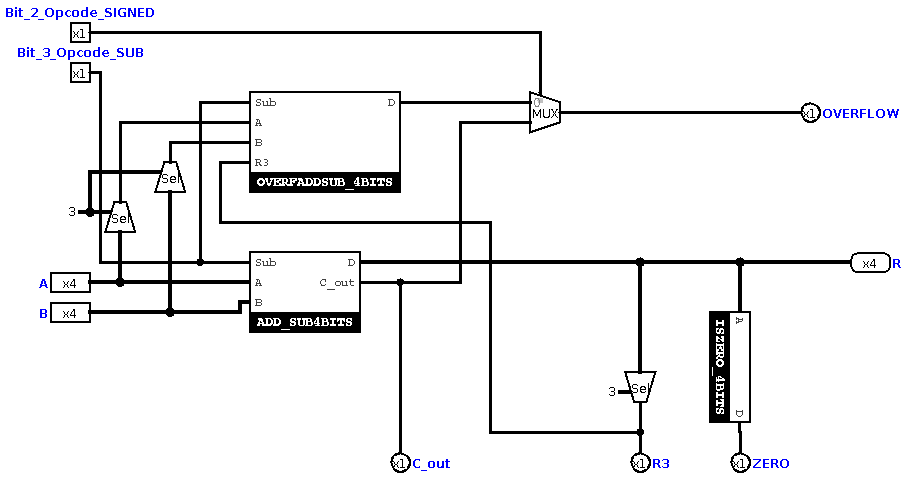
\includegraphics[width=\textwidth]{src/ADDSUB_4BITS.png}
    \captionof{figure}{Bloc ISZERO}
    \label{fig:ISZERO}
\end{figure}

\begin{figure}[H]
    \centering
    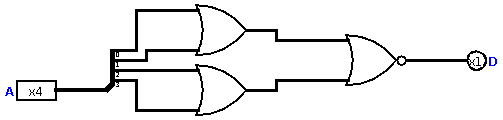
\includegraphics[width=\textwidth]{src/ISZERO_4BITS.png}
    \captionof{figure}{Bloc ISZERO}
    \label{fig:ISZERO}
\end{figure}


\begin{figure}[H]
     \centering
    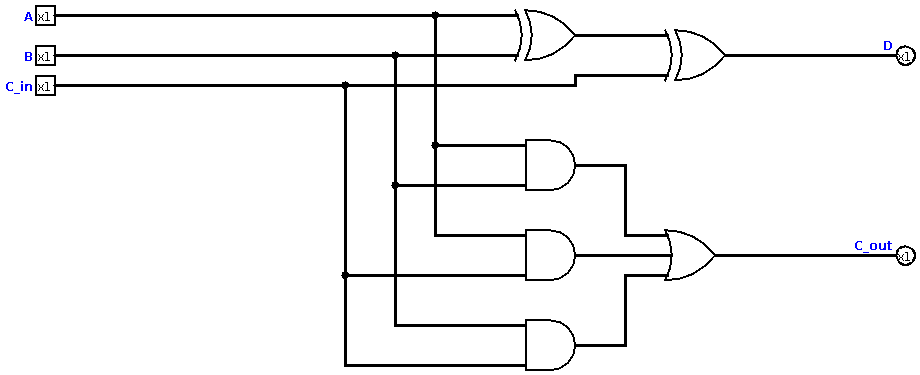
\includegraphics[width=\textwidth]{src/ADD_1BIT.png}
    \captionof{figure}{Bloc ADD 1BIT}
    \label{fig:ADD_1BIT}
\end{figure}


\begin{figure}[H]
    \centering
    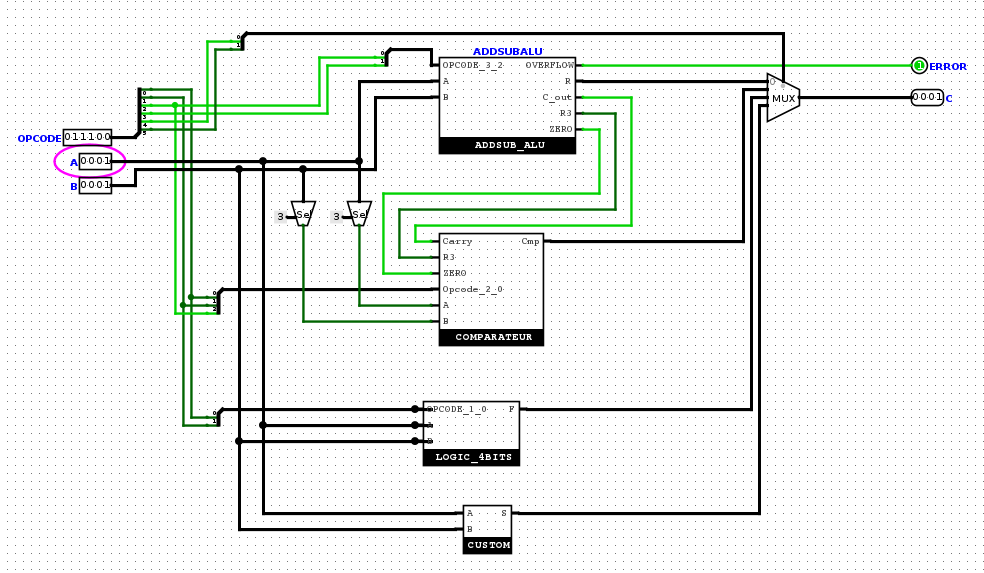
\includegraphics[width=\textwidth]{src/ALU_TEST_COMP_111.png}
    \captionof{figure}{Exemple ALU \& Comparateur}
    \label{fig:TEST_ALU_COMP_111}
\end{figure}


\begin{figure}[H]
    \centering
    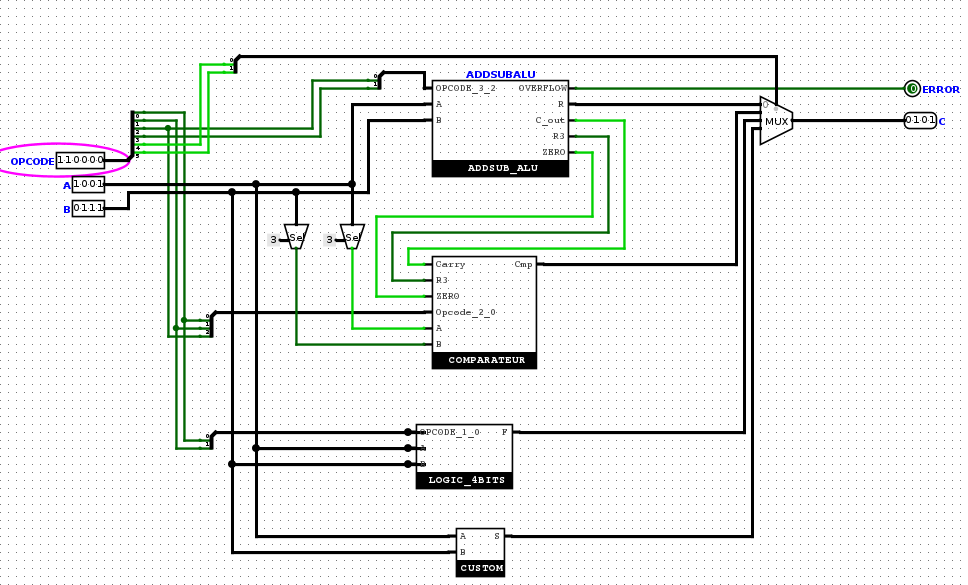
\includegraphics[width=\textwidth]{src/ALU_TEST_CUSTOM.png}
    \captionof{figure}{Exemple ALU \& CUSTOM}
    \label{fig:TEST_ALU_CUSTO}
\end{figure}


\begin{figure}[H]
    \centering
    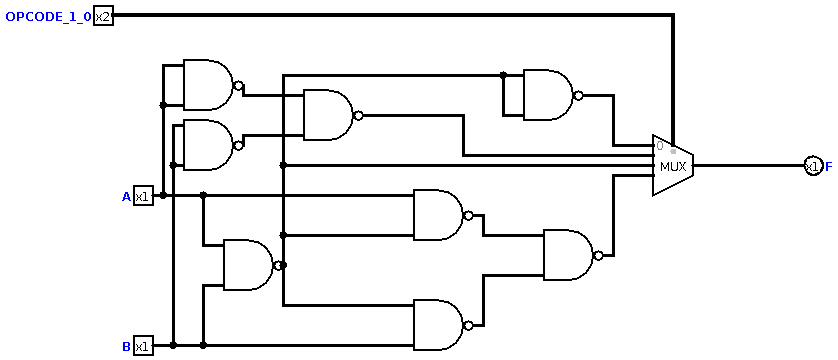
\includegraphics[width=\textwidth]{src/LOGIC_1BIT.png}
    \captionof{figure}{Circuit LOGIQUE 1BIT}
    \label{fig:LOGIQUE_1BIT}
\end{figure}


\end{document}